\section{Experiments and Results}

All experiments were conducted using Google Colab with a CPU runtime, 12.67 GB of RAM, and TensorFlow version 2.18.0. The model was trained on the noisy-clean MNIST image pairs for 15 epochs using a batch size of 128. Binary cross-entropy was used as the loss function and the Adam optimizer was employed with default parameters.

To evaluate the performance of the model, we used both quantitative metrics and visual inspection. The average Peak Signal-to-Noise Ratio (PSNR) over the first 100 test samples was 20.38 dB, and the average Structural Similarity Index (SSIM) was 0.8655. These results confirm that the model can effectively remove Gaussian noise from the input images.

Figure~\ref{fig:denoising_results} illustrates the comparison between noisy inputs, denoised outputs, and ground truth images. As seen in the visual results, the autoencoder preserves the core structure of the digits even under high noise conditions.

The training and validation loss curve, shown in Figure~\ref{fig:loss_curve}, further demonstrates that the model converges stably without signs of overfitting.

\begin{figure}[t]
  \centering
  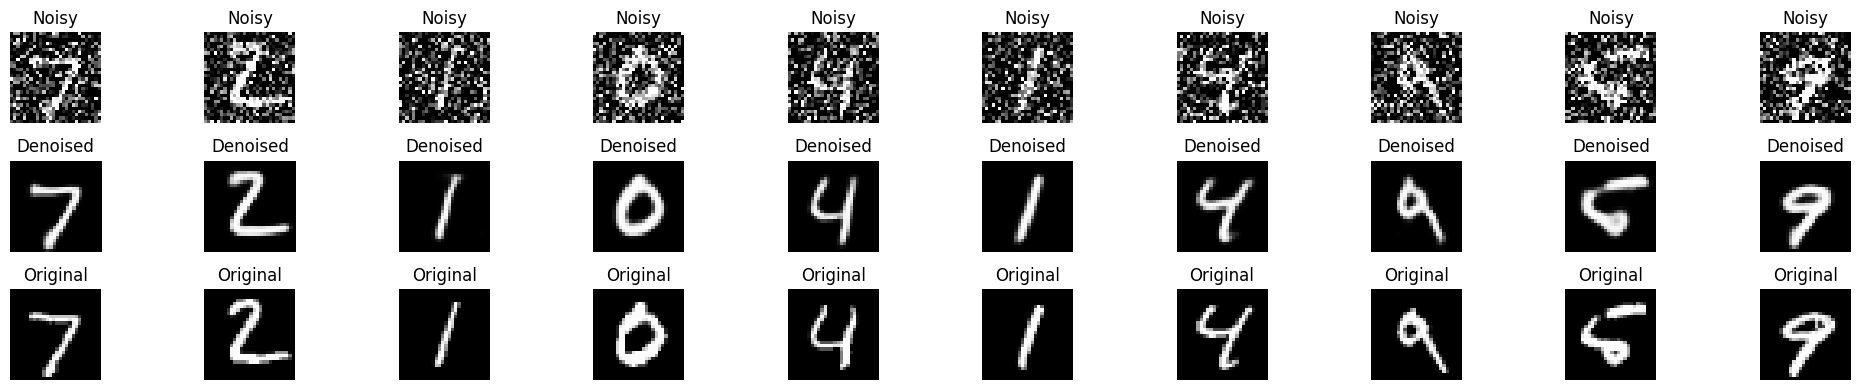
\includegraphics[width=\linewidth]{figures/denoised_examples.png}
  \caption{Denoising results of the autoencoder on MNIST test set.}
  \label{fig:denoising_results}
\end{figure}

\vspace{0.5cm}

\begin{figure}[t]
  \centering
  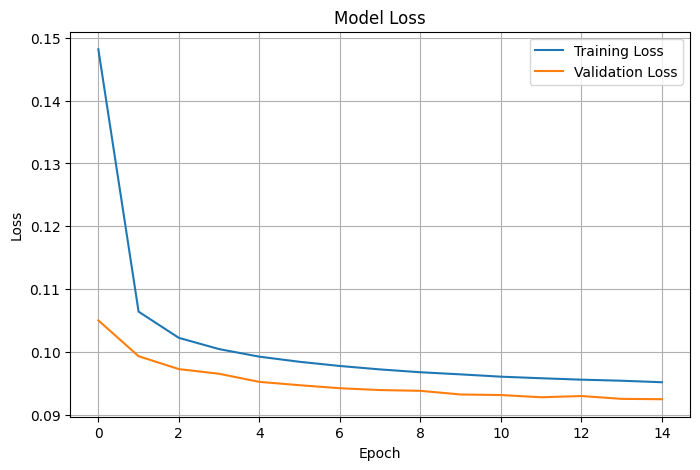
\includegraphics[width=0.8\linewidth]{figures/loss_curve.png}
  \caption{Training and validation loss over epochs.}
  \label{fig:loss_curve}
\end{figure}